\documentclass[tikz]{standalone}

\begin{document}
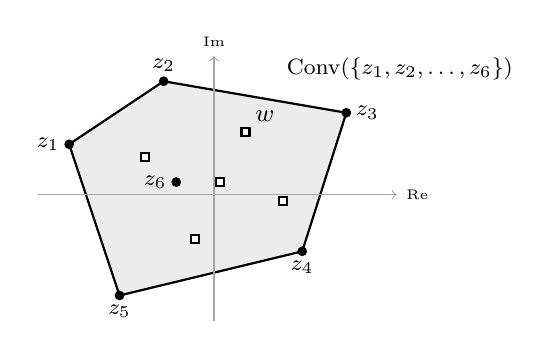
\begin{tikzpicture}[scale=0.8]
    % Marco invisible simétrico alrededor del centro del polígono (x = 0.05)
    % \useasboundingbox (-2.45,-2.1) rectangle (2.55,2.3);

    % Definición de las raíces de P(z)
    \coordinate (z1) at (-2.3, 0.8);
    \coordinate (z2) at (-0.8, 1.8);
    \coordinate (z3) at (2.1, 1.3);
    \coordinate (z4) at (1.4, -0.9); % <-- MOVIDO A LA IZQUIERDA (De 2.4 a 1.4)
    \coordinate (z5) at (-1.5, -1.6);

    % Envolvente convexa en gris claro
    \filldraw[fill=gray!15, draw=black, thick] 
        (z1) -- (z2) -- (z3) -- (z4) -- (z5) -- cycle;

    % Ejes del plano complejo (simétricos respecto al polígono)
    \draw[->, thin, gray!70] (-2.8,0) -- (2.9,0) node[right, black] {\tiny $\mathrm{Re}$};
    \draw[->, thin, gray!70] (0,-2.0) -- (0,2.2) node[above, black] {\tiny $\mathrm{Im}$};

    % Raíces de P(z) (círculos negros sólidos)
    \foreach \p/\pos/\nombre in {
        z1/left/$z_1$, 
        z2/above/$z_2$, 
        z3/right/$z_3$, 
        z4/below/$z_4$, % <-- CAMBIADO A BELOW para que no se encime con la línea
        z5/below/$z_5$
    }{
        \fill[black] (\p) circle (2.2pt) node[\pos, black] {\footnotesize \nombre};
    }

    % Raíz interior extra de P(z)
    \coordinate (z6) at (-0.6, 0.2);
    \fill[black] (z6) circle (2.2pt) node[left, black] {\footnotesize $z_6$};

    % Raíces de la derivada P'(z) (cuadrados blancos)
    \coordinate (w1) at (-1.1, 0.6);
    \coordinate (w2) at (0.5, 1.0);
    \coordinate (w3) at (1.1, -0.1);
    \coordinate (w4) at (-0.3, -0.7);
    \coordinate (w5) at (0.1, 0.2);

    \foreach \w in {w1, w2, w3, w4, w5}{
        \filldraw[fill=white, draw=black, thick] (\w) ++(-1.8pt,-1.8pt) rectangle ++(3.6pt,3.6pt);
    }

    % Etiquetas
    \node[anchor=west] at (1, 2.0) {\footnotesize $\mathrm{Conv}(\{z_{1},z_{2},\dots ,z_{6}\})$};
    \node[black, above right] at (w2) {\small $w$};
\end{tikzpicture}
\end{document} 
